% =====================================================================
%  VIGIL preprint  —  CoRL / arXiv-style single-column layout
%  (visual style modelled on the "VLK" arXiv preprint)
%
%  HOW TO COMPILE (easiest, no local install):
%    1. Go to https://overleaf.com  ->  New Project  ->  Blank Project
%    2. Replace the default main.tex with this file's contents.
%    3. Upload the four figures into the SAME project folder:
%         figure1_architecture.png  figure2_validation.png
%         figure3_kg.png            figure4_dashboard.png
%    4. Menu = pdfLaTeX. Click "Recompile". Done -> download PDF.
%
%  Then post the PDF to arXiv / attach to the Zenodo record.
% =====================================================================
\documentclass[10pt]{article}

% ---- page geometry: centred single column, CoRL-like text block ----
\usepackage[letterpaper,margin=1in]{geometry}

% ---- Times fonts give the arXiv/CoRL feel ----
\usepackage{newtxtext,newtxmath}

% ---- graphics, tables, links, captions ----
\usepackage{graphicx}
\usepackage{booktabs}
\usepackage{caption}
\usepackage[table]{xcolor}
\usepackage{titlesec}
\usepackage[colorlinks=true,allcolors=blue!55!black]{hyperref}

% ---- section headings: bold, CoRL-style ----
\titleformat{\section}{\normalfont\large\bfseries}{\thesection}{0.6em}{}
\titleformat{\subsection}{\normalfont\normalsize\bfseries}{\thesubsection}{0.6em}{}
\titlespacing*{\section}{0pt}{1.2\baselineskip}{0.4\baselineskip}

% ---- caption style ----
\captionsetup{font=small,labelfont=bf,labelsep=period}

% ---- title-block spacing ----
\title{\vspace{-1.2cm}\bfseries VIGIL: A Validation-First Research Infrastructure
for Global Infectious-Disease Intelligence}

\author{Yen-Hsiang Wang, MD, MSc \\[4pt]
{\small\itshape Graduate Institute of Medical Sciences, College of Medicine,
Taipei Medical University, Taipei 11031, Taiwan}\\[3pt]
{\small
\href{mailto:rogerwang890928@gmail.com}{rogerwang890928@gmail.com}
~$\cdot$~ ORCID~\href{https://orcid.org/0000-0003-0307-8447}{0000-0003-0307-8447}}}

\date{}

% =====================================================================
\begin{document}
\maketitle
\thispagestyle{empty}

% ---- Teaser figure (vertical concept), top of page 1 ----
\begin{figure}[h]
  \centering
  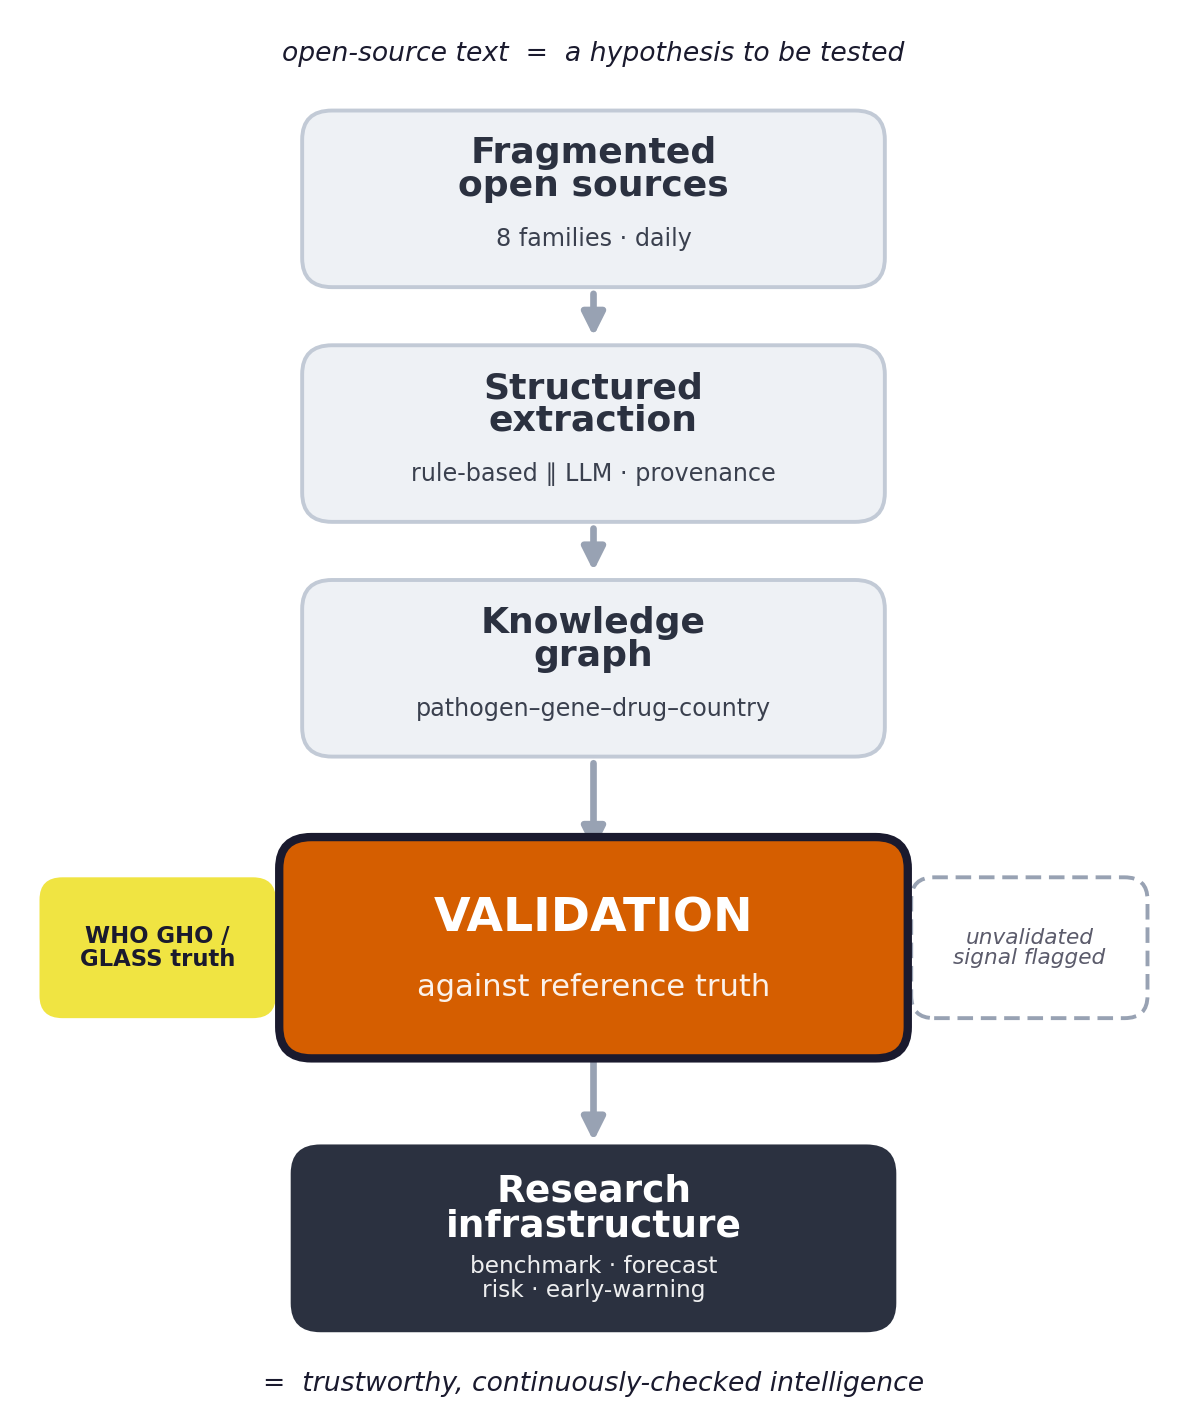
\includegraphics[width=0.52\linewidth]{fig1_architecture.png}
  \caption{VIGIL as a validation-first research infrastructure. Open-source text
  enters as fragmented signal; it is extracted to a common schema and linked into a
  knowledge graph, and then --- the pivotal step --- \emph{validated against
  independent WHO GHO/GLASS reference truth} before it is trusted. Validated signal
  becomes research infrastructure (benchmarking, forecasting, risk, early-warning);
  unvalidated signal is flagged, not acted on.}
  \label{fig:arch}
\end{figure}

% ---- Abstract block (narrowed & centred, CoRL look) ----
\begin{center}
\begin{minipage}{0.86\linewidth}
\small
\noindent\textbf{Abstract.}
Infectious-disease and antimicrobial-resistance (AMR) intelligence is increasingly
mined from open-source text --- outbreak alerts, the peer-reviewed and preprint
literature, and trial registries. But text-derived signals inherit reporting and
publication bias, and are almost never checked against independent reference truth
before they inform situational awareness. We argue that open-source
infectious-disease intelligence should be treated not as a signal to be trusted but
as a hypothesis to be \emph{validated}, and that this validation must be continuous,
reproducible, and grounded in reference surveillance data. \emph{How should
open-source infectious-disease intelligence be validated?} We answer with
\textbf{VIGIL}, a validation-first research infrastructure that collects documents
daily from eight open source families, extracts a fixed schema with a transparent
rule-based baseline and a large language model (LLM) side by side, links entities
into a knowledge graph, and --- as its primary operation --- grounds every derived
signal against WHO GHO/GLASS reference resistance data rather than asserting it. From
a snapshot of 2{,}075 documents VIGIL produced 31 pathogens, 12 resistance
mechanisms, 62 countries, and 1{,}060 knowledge-graph relations, aligned against
1{,}005 reference resistance values. Validation immediately proves its worth: across
43 countries, raw literature volume was essentially uncorrelated with measured MRSA
bloodstream-infection resistance (Spearman $\rho=0.07$), and even after
publication-normalisation the association remained weak ($\rho=0.16$) --- direct
evidence that text volume must not be read as a resistance proxy. Rather than a
weakness, this result is the point: VIGIL turns an unexamined caveat into a
measurable, continuously monitored target, and provides the standing apparatus for a
program of validation studies (LLM-extraction benchmarking, lead-time forecasting
against GLASS, and risk calibration). It is open, runs and updates daily for free,
and is archived with a citable DOI.

\vspace{0.5em}
\noindent\textbf{Keywords:} validation-first surveillance; external validation;
research infrastructure; antimicrobial resistance; large language models;
information extraction; knowledge graph; open data; Asia-Pacific.

\vspace{0.5em}
\noindent\textbf{Availability:}
Code~\href{https://github.com/Rogerking928/id-intel-platform}{github.com/Rogerking928/id-intel-platform}
~$\cdot$~ Archive/DOI~\href{https://doi.org/10.5281/zenodo.21263882}{10.5281/zenodo.21263882}
~$\cdot$~ Live demo~\href{https://id-intel-platform-4gkpazd4mhtj2upak5pzm9.streamlit.app/}{streamlit.app}
~$\cdot$~ Licence MIT.
\end{minipage}
\end{center}

\vspace{0.6em}

% =====================================================================
\section{Introduction}
Knowing where resistant pathogens and outbreaks are emerging is a fundamental
problem for global health, and antimicrobial resistance (AMR) --- associated with
millions of deaths annually and heaviest where surveillance is weakest~\cite{gbd}
--- makes it acute. The evidence is not missing; it is scattered. Every day,
national and supranational alerts, the peer-reviewed and preprint literature, and
clinical-trial registries emit open-source text about resistant organisms, in
heterogeneous formats and without a common structure. Converting this stream into
intelligence a clinician or analyst can act on requires connecting the same entities
--- pathogen, resistance mechanism, antibiotic, disease, and place --- across all of
these sources, uniformly and continuously.

Extracting this structured tuple at scale requires three things together: broad
automated ingestion of open sources, uniform entity--relation extraction, and
grounding against reference surveillance data. Prior work supplies each ingredient
in isolation, but none supplies all three. Open-source epidemic-intelligence systems
--- WHO EIOS, HealthMap, ProMED-mail, EPIWATCH --- aggregate and flag disease
events well~\cite{eios,healthmap,promed,epiwatch}, but they target outbreak
\emph{events} rather than the \emph{structured, AMR-specific}
pathogen--gene--antibiotic--country relationships that AMR research and stewardship
need, and several are proprietary or not straightforwardly reproducible. Curated
surveillance systems such as WHO GLASS provide authoritative laboratory resistance
data, but with reporting lag and limited country coverage~\cite{glass}. Large
language models (LLMs) now make structured extraction from free text feasible, but
their use in AMR surveillance raises unresolved questions of accuracy,
reproducibility, cost, and clinician trust, and there is little open, benchmarked
tooling --- particularly outside high-income, English-clinical-note
settings.% TODO before archival: add 1-3 references on LLM/NLP information extraction in public-health surveillance and on benchmarking of open LLMs.

Almost every system above produces a signal and asks the reader to trust it; few
treat \emph{validation against independent reference data} as a first-class, standing
operation. We take this to be the decisive gap, and reframe the problem accordingly:
\emph{How should open-source infectious-disease intelligence be validated ---
continuously, reproducibly, and against reference truth?} Extraction accuracy is a
means; validation is the object. We present \textbf{VIGIL} (Vigilance Intelligence
for Global Infectious-disease \& resistance Landscape), a validation-first research
infrastructure built around this question: it ingests and structures open sources
automatically, but every derived signal is grounded against WHO GHO/GLASS reference
resistance before it is reported, and each analytic module is posed as a research
question with an explicit validation design. VIGIL is released fully open-source,
runs at no cost, and carries an Asia-Pacific lens.

\noindent This paper makes four contributions:
\begin{itemize}\itemsep2pt
  \item \textbf{Validation as the primary operation.} VIGIL grounds every
  text-derived signal against independent WHO GHO/GLASS reference resistance data
  rather than asserting it, making validation --- not extraction --- the object of
  study.
  \item \textbf{An open, provenance-complete pipeline} that ingests eight open source
  families daily and records full provenance (raw text, source, timestamp, and, per
  extraction, the extractor, model, and prompt version), turning extraction itself
  into a reproducibly benchmarkable object with a transparent rule-based baseline and
  an LLM run side by side on identical inputs.
  \item \textbf{A knowledge graph and a suite of validation-first modules} (trends,
  forecasting, novelty, risk, outbreak, and an extraction benchmark), each framed as
  research question $\rightarrow$ validation design $\rightarrow$ current result
  rather than as a product feature.
  \item \textbf{Evidence that validation is necessary}, obtained by turning the
  infrastructure on itself: text volume is essentially uninformative about measured
  resistance --- reframing an unexamined caveat into a measurable, continuously
  monitored target and a research program.
\end{itemize}

\begin{figure}[t]
  \centering
  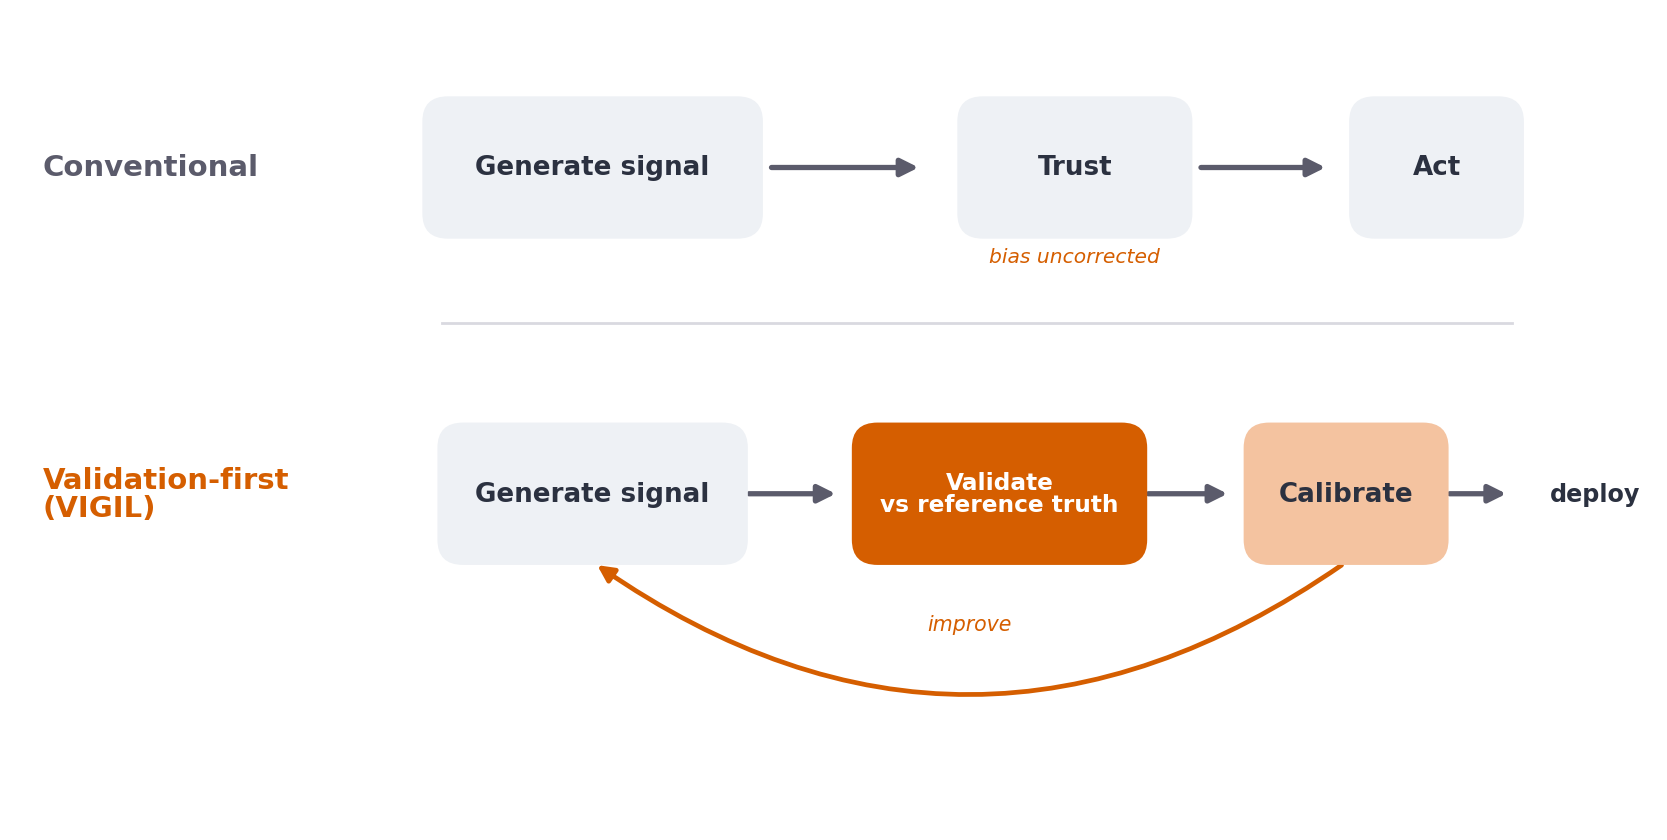
\includegraphics[width=\linewidth]{fig2_paradigm.png}
  \caption{The design shift VIGIL embodies. Conventional open-source intelligence
  \emph{generates a signal and trusts it}, carrying uncorrected reporting and
  publication bias into action. A validation-first system instead treats each signal
  as provisional: it is validated against independent reference truth, used to
  calibrate the method, and only then deployed --- a continuous loop rather than a
  one-way pipeline.}
  \label{fig:paradigm}
\end{figure}

% =====================================================================
\section{Implementation}

\subsection{Overview and architecture}
VIGIL follows a linear, auditable pipeline: \textbf{collect $\rightarrow$ extract
$\rightarrow$ entities/relations $\rightarrow$ analyse $\rightarrow$ serve}
(Figure~\ref{fig:arch}). Documents are stored in a single SQLite database. Every
document retains its raw text, source, URL, and fetch timestamp; every extraction
retains the extractor name, model version, prompt version, and raw output. This
provenance makes each analytic result traceable to source text and supports
head-to-head comparison of extractors.

\subsection{Data sources}
Eight source families are configured (Table~\ref{tab:sources}), each accessed
through public APIs or feeds and de-duplicated so that only new records are appended
on each run. Sources span official alerts (WHO DON, CDC, ECDC, UKHSA), the
literature (PubMed~\cite{eutils}, bioRxiv/medRxiv via Europe PMC~\cite{europepmc}),
trials (ClinicalTrials.gov~\cite{ctgov}), and reference resistance data
(WHO GHO/GLASS~\cite{gho,glass}).

\begin{table}[h]
  \centering
  \caption{Configured data sources.}
  \label{tab:sources}
  \small
  \begin{tabular}{lll}
    \toprule
    \textbf{Source} & \textbf{Type} & \textbf{Access} \\
    \midrule
    WHO Disease Outbreak News & Official outbreak alerts & JSON (OData) API \\
    US CDC & Alerts / MMWR / newsroom & RSS \\
    ECDC & European communicable-disease news & RSS \\
    UK Health Security Agency & News \& guidance & GOV.UK Atom feed \\
    PubMed & Peer-reviewed literature & NCBI E-utilities \\
    bioRxiv / medRxiv & Preprints & Europe PMC REST API \\
    ClinicalTrials.gov & Trial registrations & API v2 \\
    WHO GHO / GLASS & Reference resistance indicators & GHO OData API \\
    \bottomrule
  \end{tabular}
\end{table}

\subsection{Information extraction}
Two extractors return an identical schema. The \textbf{rule-based} extractor
applies frozen controlled vocabularies (a versioned codebook) with word-boundary
matching, country-alias canonicalisation, and assertion/negation handling; it is
free, offline, deterministic, and serves as the benchmark baseline. The optional
\textbf{LLM} extractor (Google Gemini in the current build; the interface is
model-agnostic) is prompted to return the same JSON schema. Because both outputs
are stored per document, VIGIL supports a direct, reproducible comparison of
methods --- for example, on a paper describing altered ceftazidime-avibactam
resistance, the LLM recovered specific alleles (KPC-234, NDM-1) and plasmid context
that the dictionary baseline did not.

\subsection{A suite of validation-first modules}
Entity co-occurrence within a document generates
Pathogen\,$\rightarrow$\,Country\,$\rightarrow$\,Gene\,$\rightarrow$\,Antibiotic\,$\rightarrow$\,Disease
relations, queryable as a graph. On top of the graph and entity tables, VIGIL exposes
its analytics not as product features but as a suite of modules, each posed as a
\emph{research question} with an explicit \emph{validation design} and an honestly
reported \emph{current status} (Table~\ref{tab:modules}). This framing is deliberate:
it makes the infrastructure's job the continual production \emph{and checking} of
surveillance signals, and holds every module accountable to reference truth rather
than to face validity.

\begin{table}[h]
  \centering
  \caption{VIGIL's validation-first modules, each framed as a research question with
  a validation design and its current status. Status is reported honestly: several
  modules are infrastructure-ready but await accumulated history or expert labels.}
  \label{tab:modules}
  \footnotesize
  \renewcommand{\arraystretch}{1.25}
  \begin{tabular}{@{}p{2.0cm}p{3.5cm}p{4.0cm}p{3.5cm}@{}}
    \toprule
    \textbf{Module} & \textbf{Research question} & \textbf{Validation design} & \textbf{Current status} \\
    \midrule
    Extraction benchmark & Do a transparent rule-based extractor and an LLM agree, and which is more accurate? & Clinician-annotated gold standard; per-field F1 and inter-annotator $\kappa$; frozen codebook and leakage controls & Infrastructure and \texttt{annotations} table ready; gold set not yet annotated \\
    Construct validity (risk) & Does a text-derived AMR signal reflect \emph{measured} resistance? & Cross-sectional Spearman vs WHO GHO MRSA / \textit{E.\ coli} BSI resistance; raw vs publication-normalised & $\rho=0.07$ raw, $0.16$ normalised across 43 countries (Fig.~\ref{fig:valid}) \\
    Outbreak & Does literature signal anticipate \emph{officially reported} outbreaks? & Source-separated: outcomes from official alerts, features from literature; rank-AUC & Qualitative negative; precise AUC to be re-run on the current snapshot \\
    Forecasting & Is discussion volume predictable, and does it lead reference surveillance? & Transparent baseline + rolling backtest; planned lead-time evaluation vs GLASS & Prototype with backtest; lead-time pending longer history \\
    Novelty & Which entity combinations are genuinely new? & Flag combinations never previously co-occurring in the dated corpus & Implemented; precision pending expert review \\
    Trends / emerging signal & What is rising fastest, and where? & Growth-rate and emerging-signal detection over the dated corpus & Implemented; preliminary (young corpus) \\
    \bottomrule
  \end{tabular}
\end{table}

\subsection{Validation design}
Analytics are grounded in reference data rather than asserted. WHO GHO/GLASS
resistance indicators (proportion of MRSA and third-generation-cephalosporin-
resistant \textit{E.\ coli} bloodstream infections) are ingested automatically as
ground truth. Construct validity is assessed cross-sectionally against these values.
The outbreak task deliberately separates sources --- outcomes are taken from
official alerts (WHO/CDC/ECDC/UKHSA) while features derive from the literature
stream --- to avoid circularity. A frozen annotation codebook and an
\texttt{annotations} table support a planned clinician-annotated extraction
benchmark under leakage controls.

\subsection{Availability and reproducibility}
VIGIL is open-source (MIT), archived on Zenodo with a DOI, deployed as a public
live instance (Appendix~A), and updated daily at no cost via continuous integration.
Code, the codebook, and the schema are versioned; a single command reproduces the
pipeline.

% =====================================================================
\section{Results}

\subsection{Corpus}
The analysed snapshot contained 2{,}075 extracted documents. Seven sources
contributed actively (CDC $n=1{,}828$; preprints $n=116$; PubMed $n=54$;
ClinicalTrials $n=37$; UKHSA $n=20$; ECDC $n=10$; WHO DON $n=10$; Figure~\ref{fig:corpus}a),
spanning research articles, outbreak alerts, AMR reports, guidelines, and trials
(Figure~\ref{fig:corpus}b); the GLASS ingestion path is included but was not
populated in this snapshot. Extraction yielded 31 distinct pathogens (including the
priority phenotypes MRSA, VRE, CRE, CRAB, and \textit{Candida auris}), 12 resistance
genes/mechanisms, 23 antibiotics, 62 countries, and 1{,}060 knowledge-graph
relations. The WHO GHO ingestion added 1{,}005 reference resistance values spanning
103 countries and 2016--2023.

\begin{figure}[h]
  \centering
  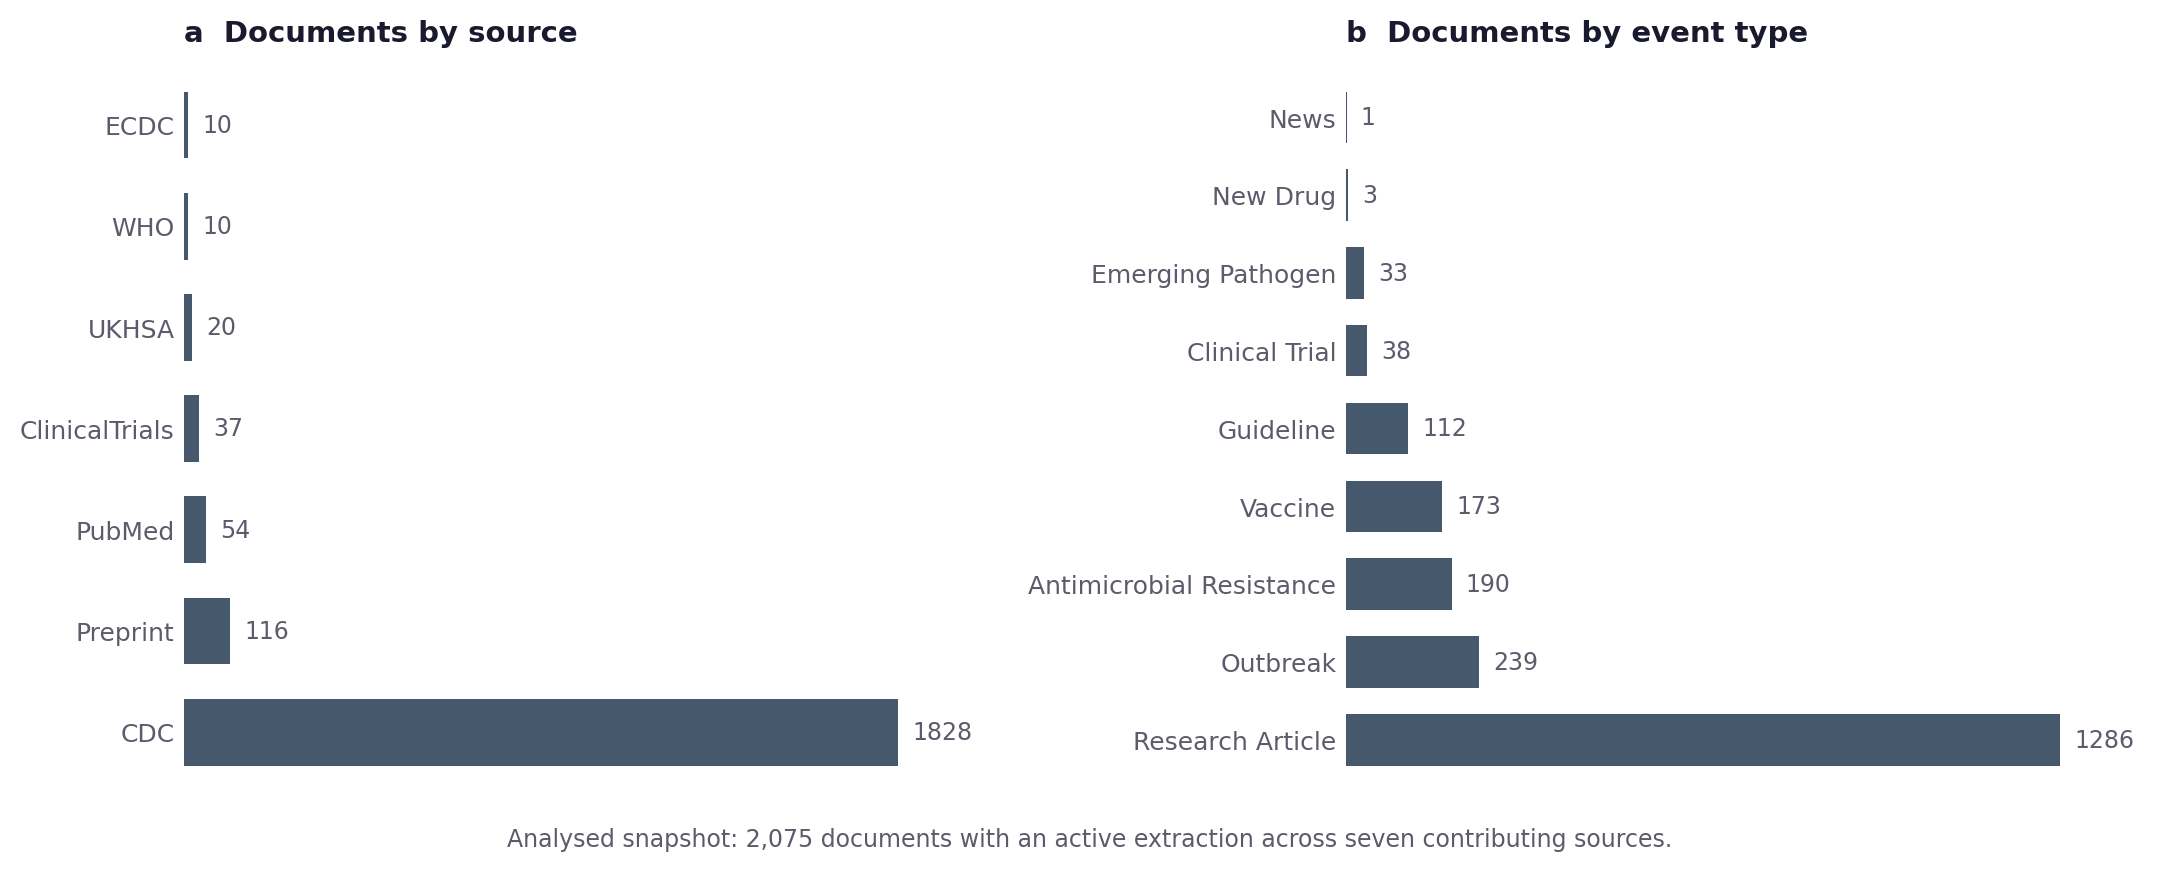
\includegraphics[width=\linewidth]{fig2_corpus.png}
  \caption{Composition of the analysed corpus. (a)~Documents by source; official
  alerts, literature, preprints, and trials contribute at very different volumes.
  (b)~Documents by extracted event type. Counts are for the 2{,}075 documents with
  an active extraction.}
  \label{fig:corpus}
\end{figure}

\subsection{Extraction and knowledge graph}
Structured extraction reproduced expected AMR concepts across pathogens, resistance
mechanisms, and antibiotics (Figure~\ref{fig:landscape}), and, for the LLM extractor,
recovered fine-grained resistance alleles absent from the baseline dictionary. Graph
queries returned interpretable chains --- for example, around carbapenem resistance
the platform linked carbapenemase genes (OXA-48, KPC, NDM) to the
Enterobacterales and non-fermenters that carry them, each edge traceable to the
underlying documents (Figure~\ref{fig:kg}).

\begin{figure}[h]
  \centering
  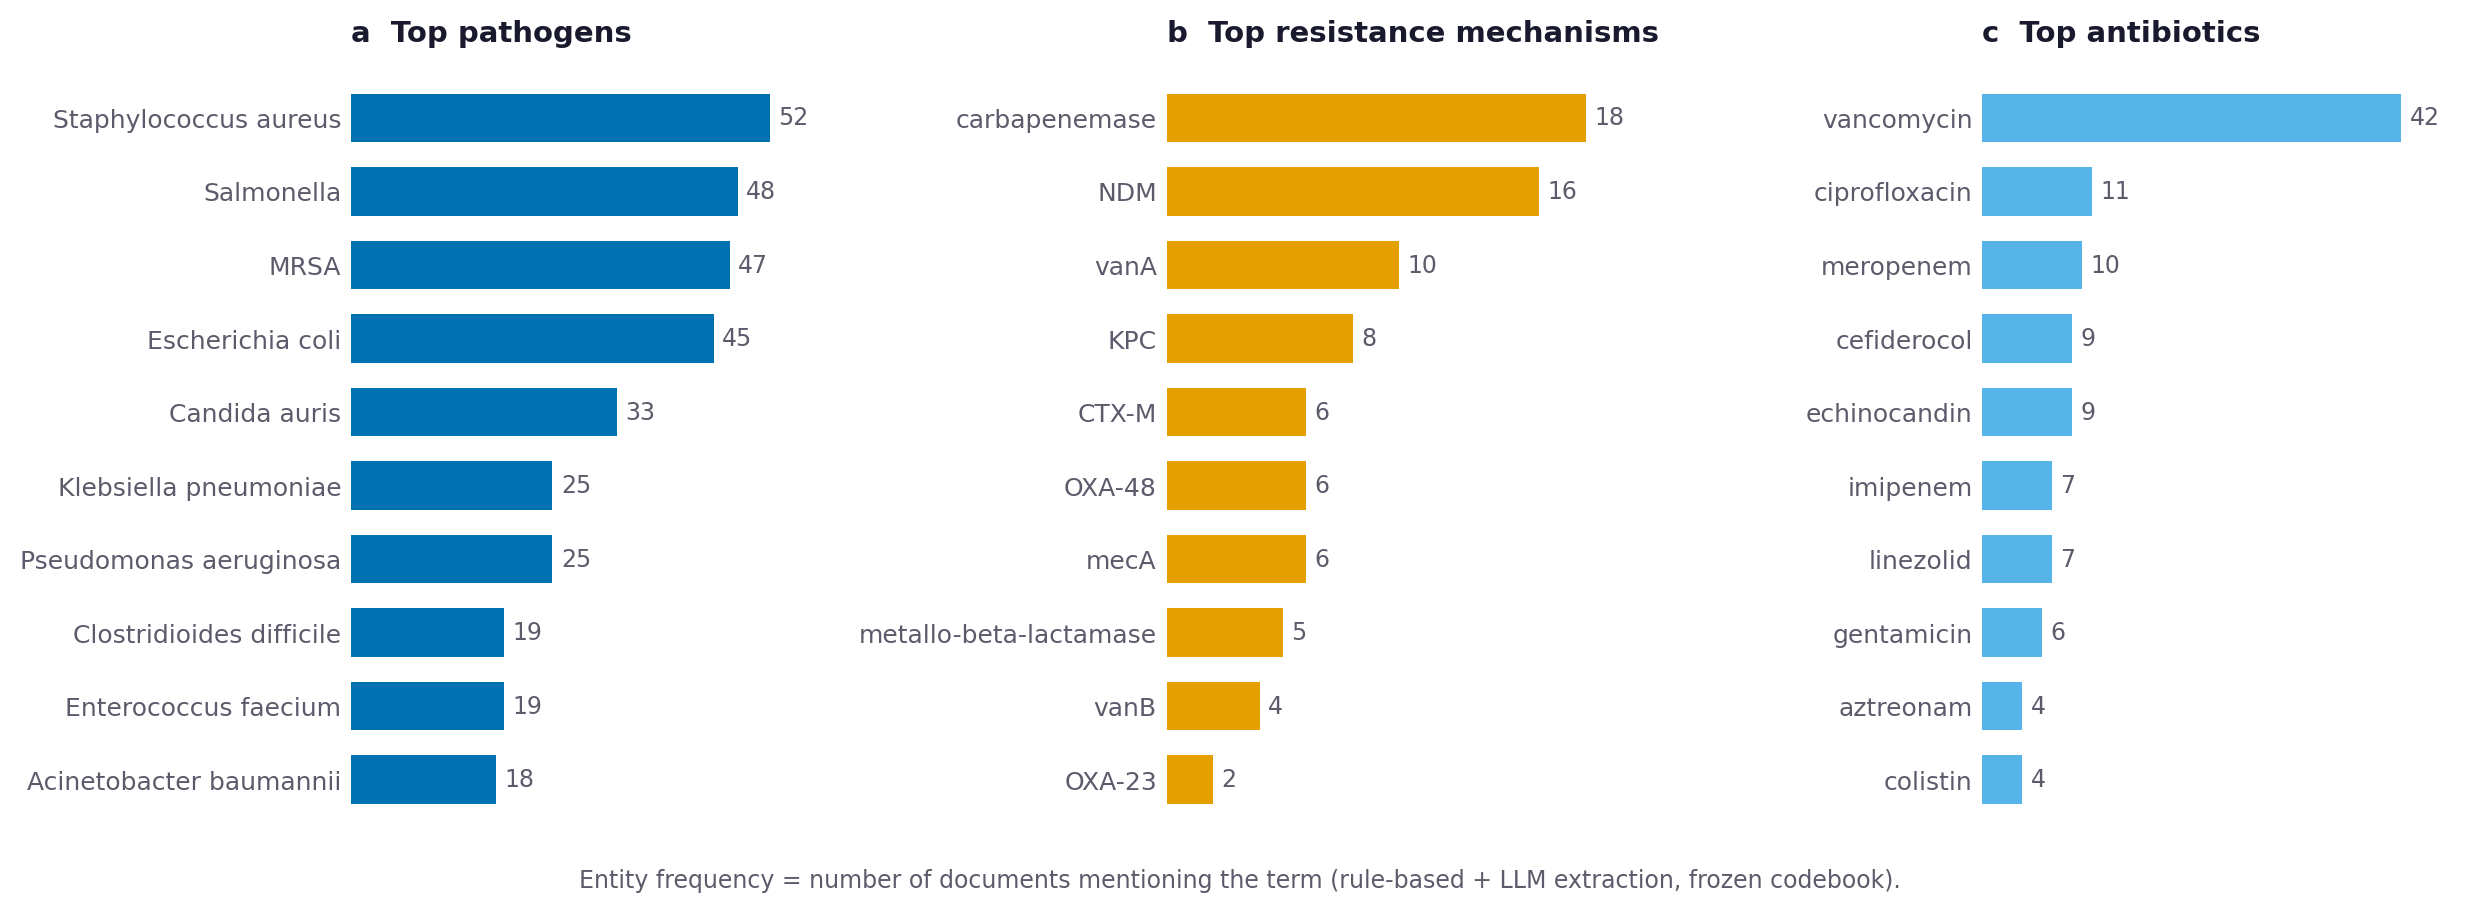
\includegraphics[width=\linewidth]{fig3_landscape.png}
  \caption{The AMR entity landscape VIGIL extracts. Most-mentioned (a)~pathogens,
  (b)~resistance mechanisms, and (c)~antibiotics, by number of documents. The
  priority phenotypes and carbapenemase genes that dominate current AMR concern are
  surfaced directly from open-source text.}
  \label{fig:landscape}
\end{figure}

\begin{figure}[h]
  \centering
  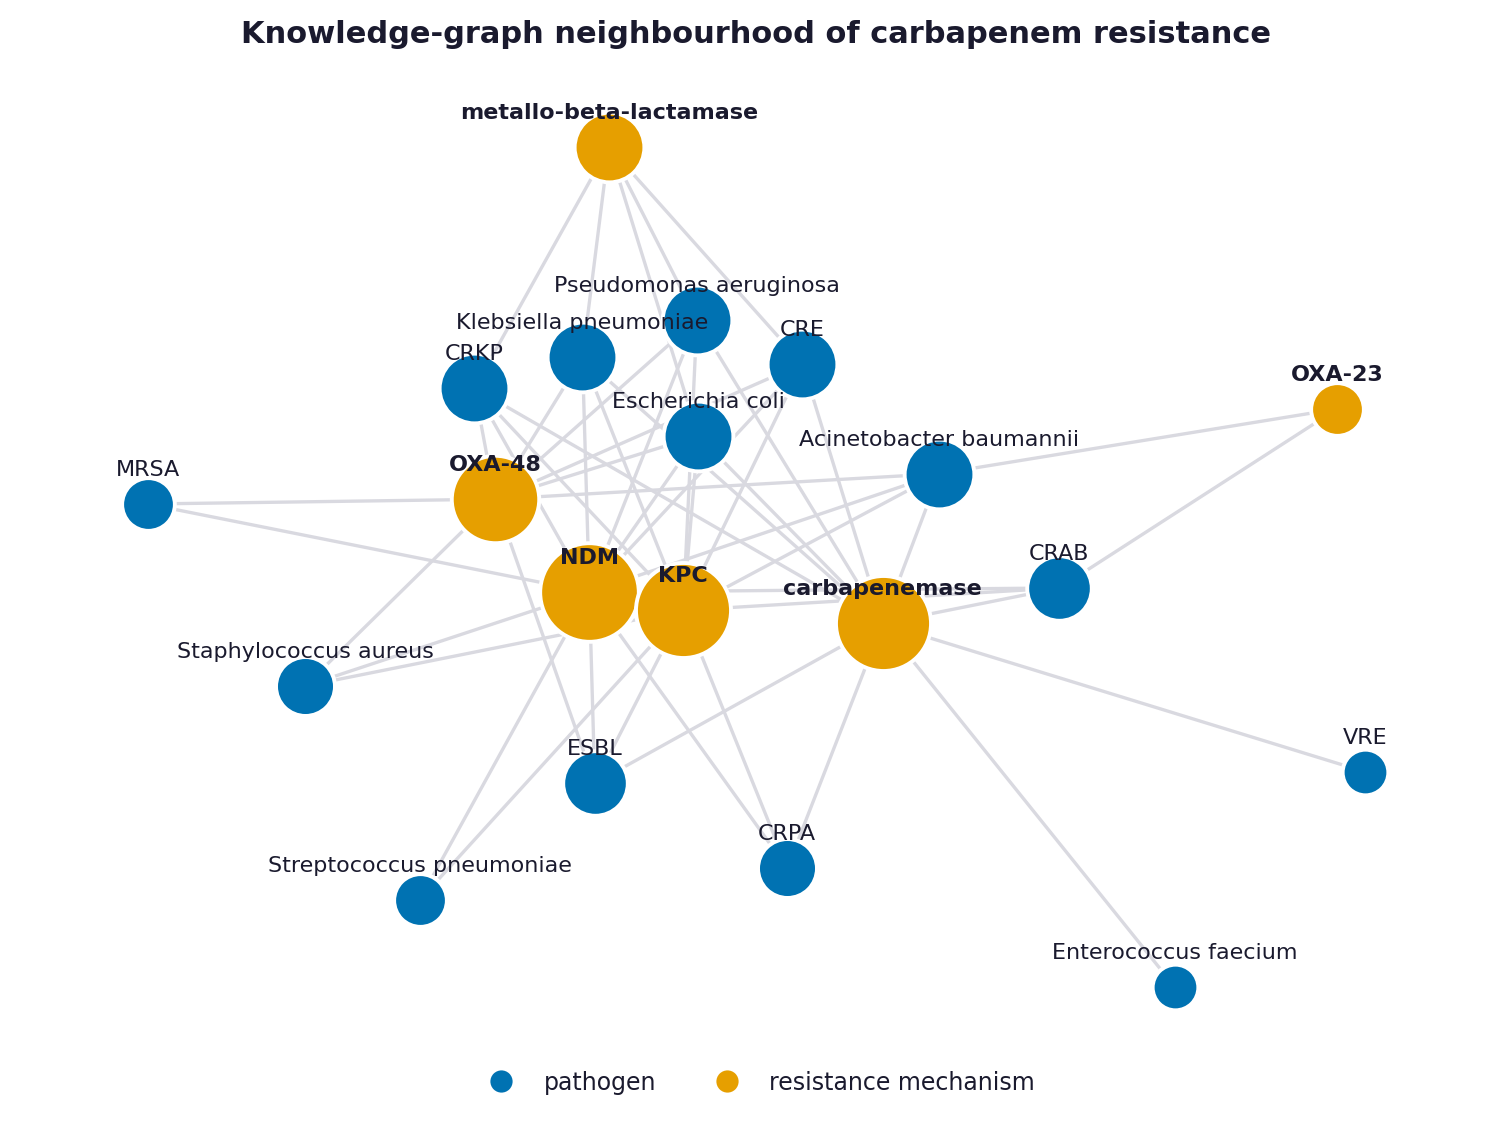
\includegraphics[width=0.82\linewidth]{fig4_kg.png}
  \caption{Knowledge-graph neighbourhood of carbapenem resistance in the corpus:
  carbapenemase genes (orange) and the pathogens (red) they co-occur with; node size
  scales with degree. Every edge is traceable to source documents.}
  \label{fig:kg}
\end{figure}

\subsection{Preliminary validation}
Across the 43 countries with both a platform AMR signal and a WHO GHO MRSA value,
raw AMR-document volume was essentially uncorrelated with measured resistance
(Spearman $\rho=0.07$), and a publication-normalised AMR share recovered only a weak
positive association ($\rho=0.16$; Figure~\ref{fig:valid}) --- consistent with
document volume reflecting research output rather than disease burden, and with
normalisation partially recovering signal. The country-level signal is sparse: most
countries contribute only a handful of AMR-tagged documents, so these are
proof-of-concept results that are expected to sharpen as the corpus accumulates. A
complementary outbreak analysis --- which deliberately separates official-alert
outcomes from literature-derived features --- likewise found that literature signal
did not track where outbreaks were officially reported, which concentrated in
lower-resource, lower-literature settings. Even at this stage, the platform makes
the surveillance gap explicit and measurable rather than hidden.

\begin{figure}[h]
  \centering
  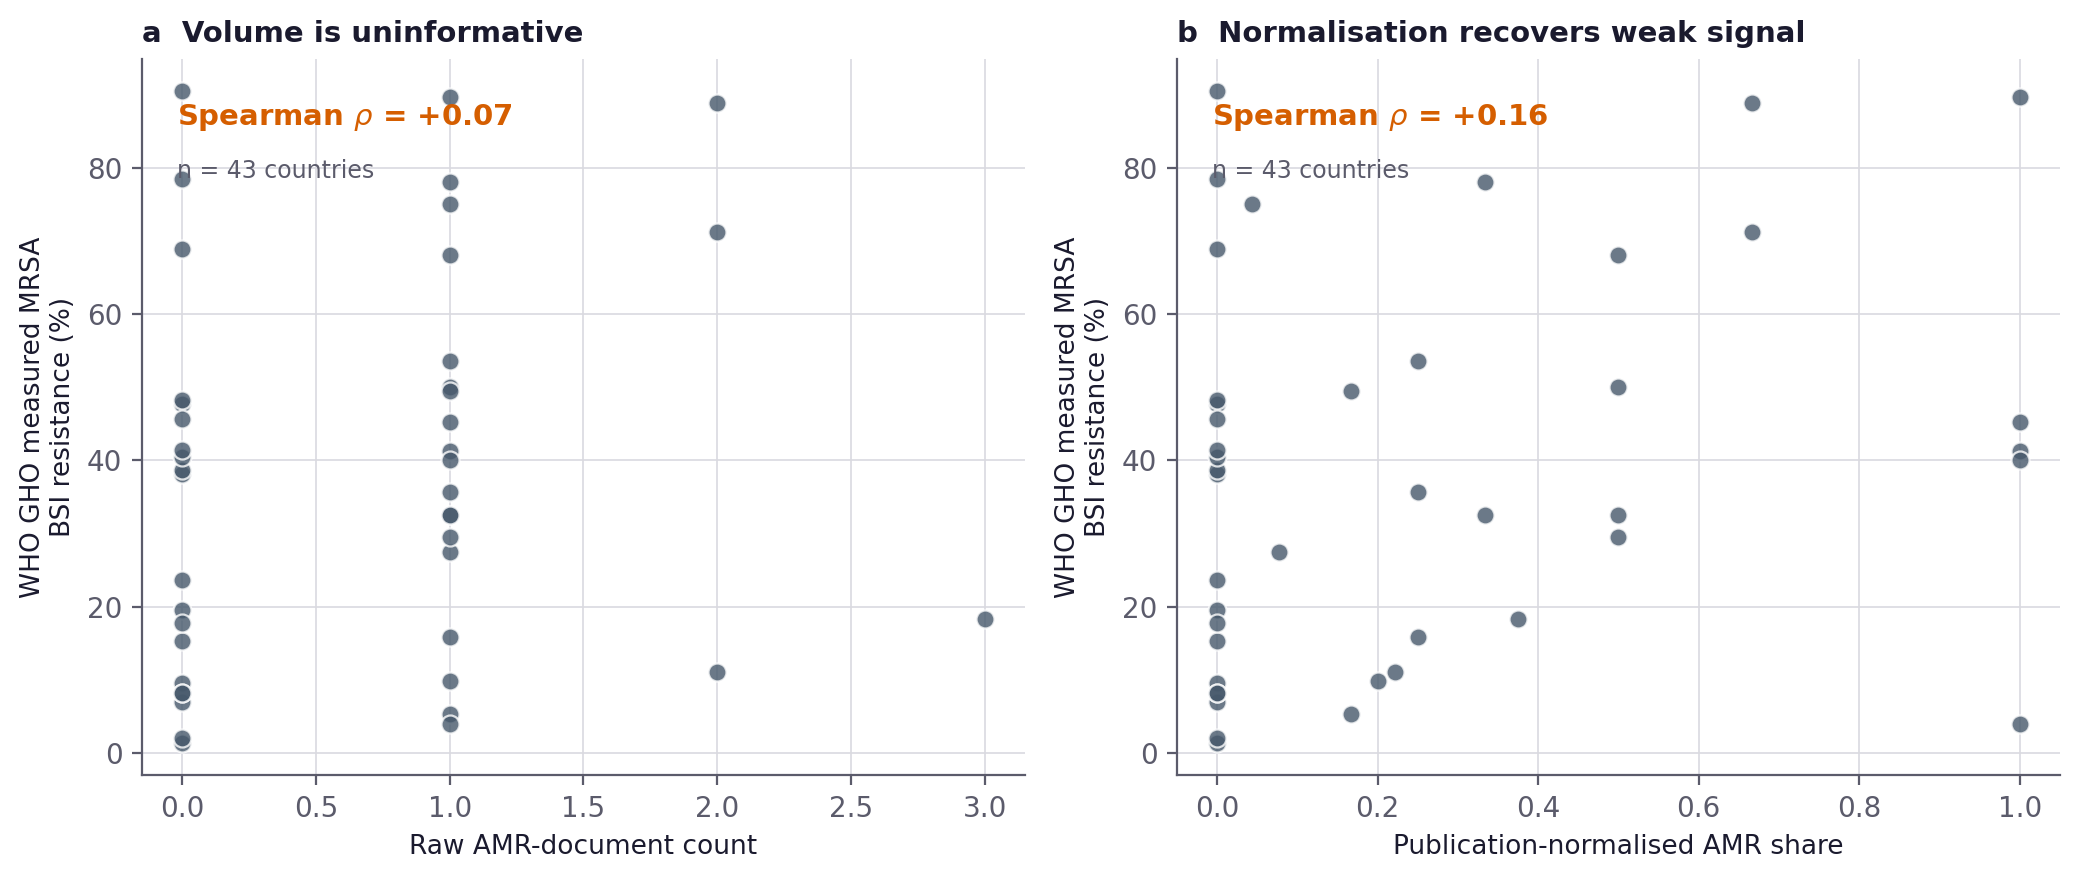
\includegraphics[width=\linewidth]{fig5_validation.png}
  \caption{Construct validity against independent reference data, across 43 countries.
  (a)~Raw AMR-document count versus WHO GHO measured MRSA bloodstream-infection
  resistance is essentially uncorrelated (Spearman $\rho=0.07$); (b)~a
  publication-normalised AMR share recovers only a weak positive association
  ($\rho=0.16$). Text volume alone does not track measured resistance --- a
  quantification of the global surveillance gap.}
  \label{fig:valid}
\end{figure}

% =====================================================================
\section{Discussion}
VIGIL complements, rather than duplicates, existing open-source
epidemic-intelligence systems: where those emphasise outbreak-event detection,
VIGIL emphasises \textbf{structured, AMR-specific extraction, a knowledge graph, and
validation against reference resistance data}, all fully open and reproducible. Its
most striking early observation --- that raw open-source literature signal is
uncorrelated with measured resistance and inversely associated with where outbreaks
are officially reported --- is itself a substantive finding: na\"ive text-volume
indicators would misrank global risk, and any credible early-warning model must
correct for reporting and publication bias. By quantifying this gap against WHO
reference data, VIGIL turns a known caveat into a measurable target.

The platform is also designed as research infrastructure. Because it stores both
rule-based and LLM outputs with full provenance and ships a frozen annotation
codebook, it directly enables a clinician-annotated benchmark of open LLMs for AMR
extraction, and its accumulating time series supports early-warning modelling with
lead-time evaluation against GLASS. Its Asia-Pacific focus addresses a region
under-represented in existing tools.

More broadly, we believe \textbf{validation-first surveillance should become a
fundamental design principle for the next generation of infectious-disease
intelligence systems}: as automated extraction and large language models make it
trivial to \emph{generate} signals from open text, the scarce and decisive capability
is no longer generation but the standing infrastructure to validate, calibrate, and
continuously re-check those signals against reference truth (Figure~\ref{fig:paradigm}).
VIGIL is one concrete instance of that principle; we hope it is among the first of
many.

% =====================================================================
\section{Limitations}
The corpus is young and unevenly dated (Figure~\ref{fig:growth}), so trend,
forecasting, and novelty analytics are preliminary and strengthen with accumulated
history. Text-derived geolocation reflects where topics are reported or studied, not
confirmed case counts, and is subject to reporting and publication bias (which the
platform surfaces rather than conceals).

\begin{figure}[h]
  \centering
  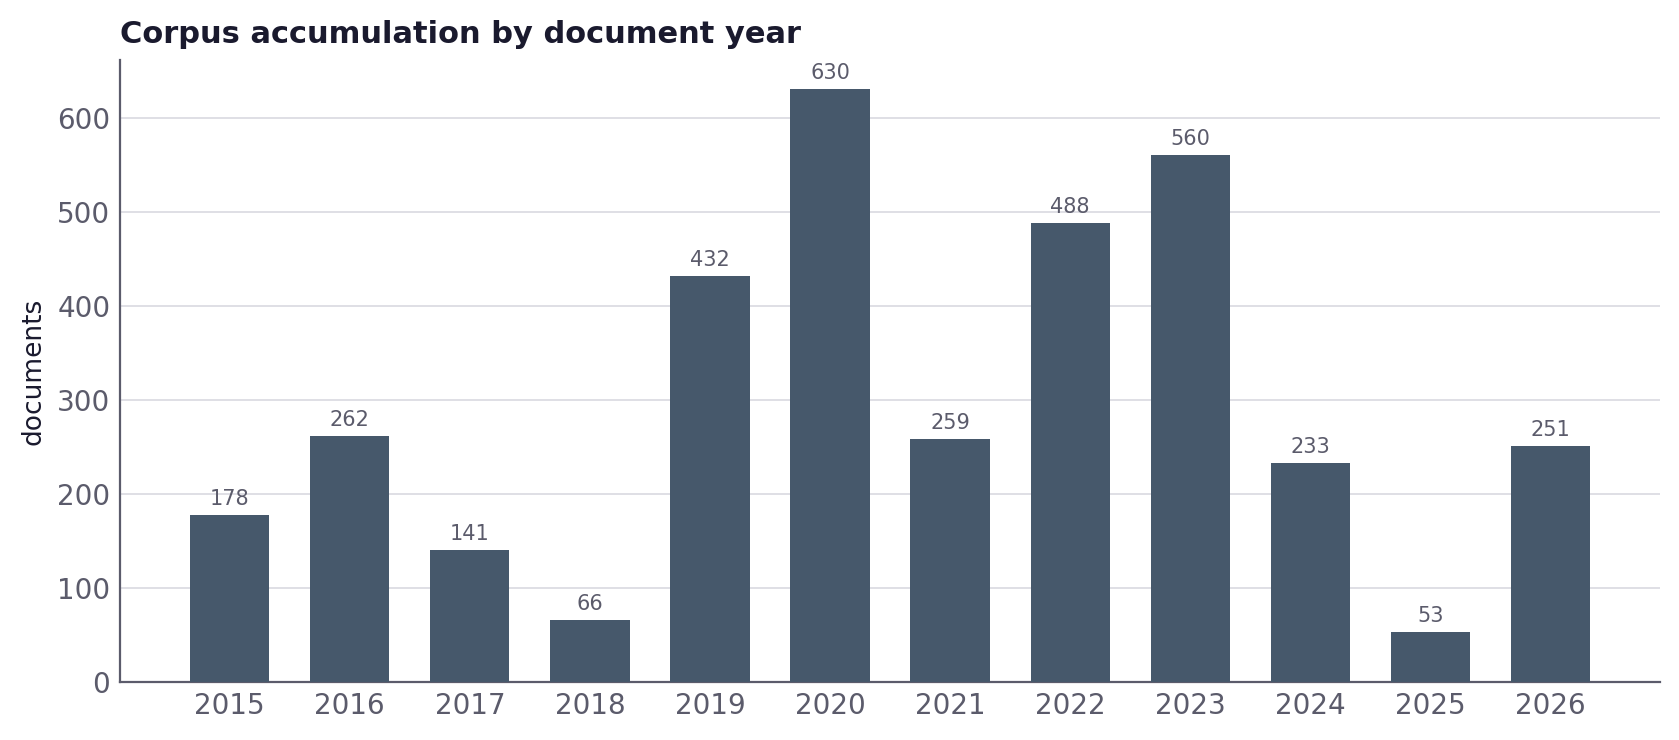
\includegraphics[width=0.72\linewidth]{fig6_growth.png}
  \caption{Documents by document year in the corpus. Coverage is concentrated in
  recent years and accumulates daily; longitudinal analytics gain power as the
  historical series lengthens.}
  \label{fig:growth}
\end{figure}
Reference coverage is incomplete: WHO GHO does not list some territories, including
Taiwan (a listing limitation of the reference source, not a platform merge), and
lacks values for several countries on these indicators. LLM extraction is currently
constrained by free-tier throughput. Finally, the extraction benchmark awaits full
clinician annotation and a second annotator for reliability estimation.

% =====================================================================
\section{Conclusion}
VIGIL is an open, validation-first platform that converts open-source
infectious-disease and AMR text into structured, citable intelligence, and a
foundation for a program of methodological studies. It is freely available, runs and
updates at no cost, and is archived with a DOI for reuse and citation.

% =====================================================================
\section*{Declarations}
\small
\textbf{Data and code availability:} all code and the annotated schema are available
on GitHub and archived on Zenodo (DOI: 10.5281/zenodo.21263882); data derive from
public open-source APIs. \textbf{Funding:} none. \textbf{Competing interests:} none
declared. \textbf{Ethics:} the platform uses only open-source, aggregate/public data
and no individual patient data. \textbf{Author contributions:} YHW conceived,
designed, implemented, and wrote the work.
\normalsize

% =====================================================================
\begin{thebibliography}{10}
\small
\bibitem{gbd}
Antimicrobial Resistance Collaborators. Global burden of bacterial antimicrobial
resistance in 2019: a systematic analysis. \textit{Lancet}. 2022;399(10325):629--655.

\bibitem{glass}
World Health Organization. Global Antimicrobial Resistance and Use Surveillance
System (GLASS). Geneva: WHO. Available from:
\url{https://www.who.int/initiatives/glass}

\bibitem{eios}
World Health Organization. Epidemic Intelligence from Open Sources (EIOS). Geneva:
WHO. Available from: \url{https://www.who.int/initiatives/eios}

\bibitem{healthmap}
Freifeld CC, Mandl KD, Reis BY, Brownstein JS. HealthMap: global infectious disease
monitoring through automated classification and visualization of Internet media
reports. \textit{J Am Med Inform Assoc}. 2008;15(2):150--157.

\bibitem{promed}
International Society for Infectious Diseases. ProMED-mail. Available from:
\url{https://promedmail.org}

\bibitem{epiwatch}
MacIntyre CR, et al. EPIWATCH: open-source epidemic observatory. Sydney: UNSW.
Available from: \url{https://www.epiwatch.org}

\bibitem{gho}
World Health Organization. Global Health Observatory OData API. Geneva: WHO.
Available from: \url{https://www.who.int/data/gho/info/gho-odata-api}

\bibitem{eutils}
National Center for Biotechnology Information. Entrez Programming Utilities
(E-utilities). Bethesda (MD): NCBI. Available from:
\url{https://www.ncbi.nlm.nih.gov/books/NBK25501/}

\bibitem{europepmc}
Europe PMC Consortium. Europe PMC RESTful Web Service. Available from:
\url{https://europepmc.org/RestfulWebService}

\bibitem{ctgov}
National Library of Medicine. ClinicalTrials.gov API. Bethesda (MD): NLM. Available
from: \url{https://clinicaltrials.gov/data-api/api}
\end{thebibliography}

% =====================================================================
\section*{Appendix A. Live instance}
\small
The infrastructure runs as a public, daily-updated web instance
(\href{https://id-intel-platform-4gkpazd4mhtj2upak5pzm9.streamlit.app/}{streamlit.app}),
which exposes every module in Table~\ref{tab:modules} together with the search,
knowledge-graph, heatmap, annotation, and benchmark tools (Figure~\ref{fig:dash}).
\normalsize
\begin{figure}[h]
  \centering
  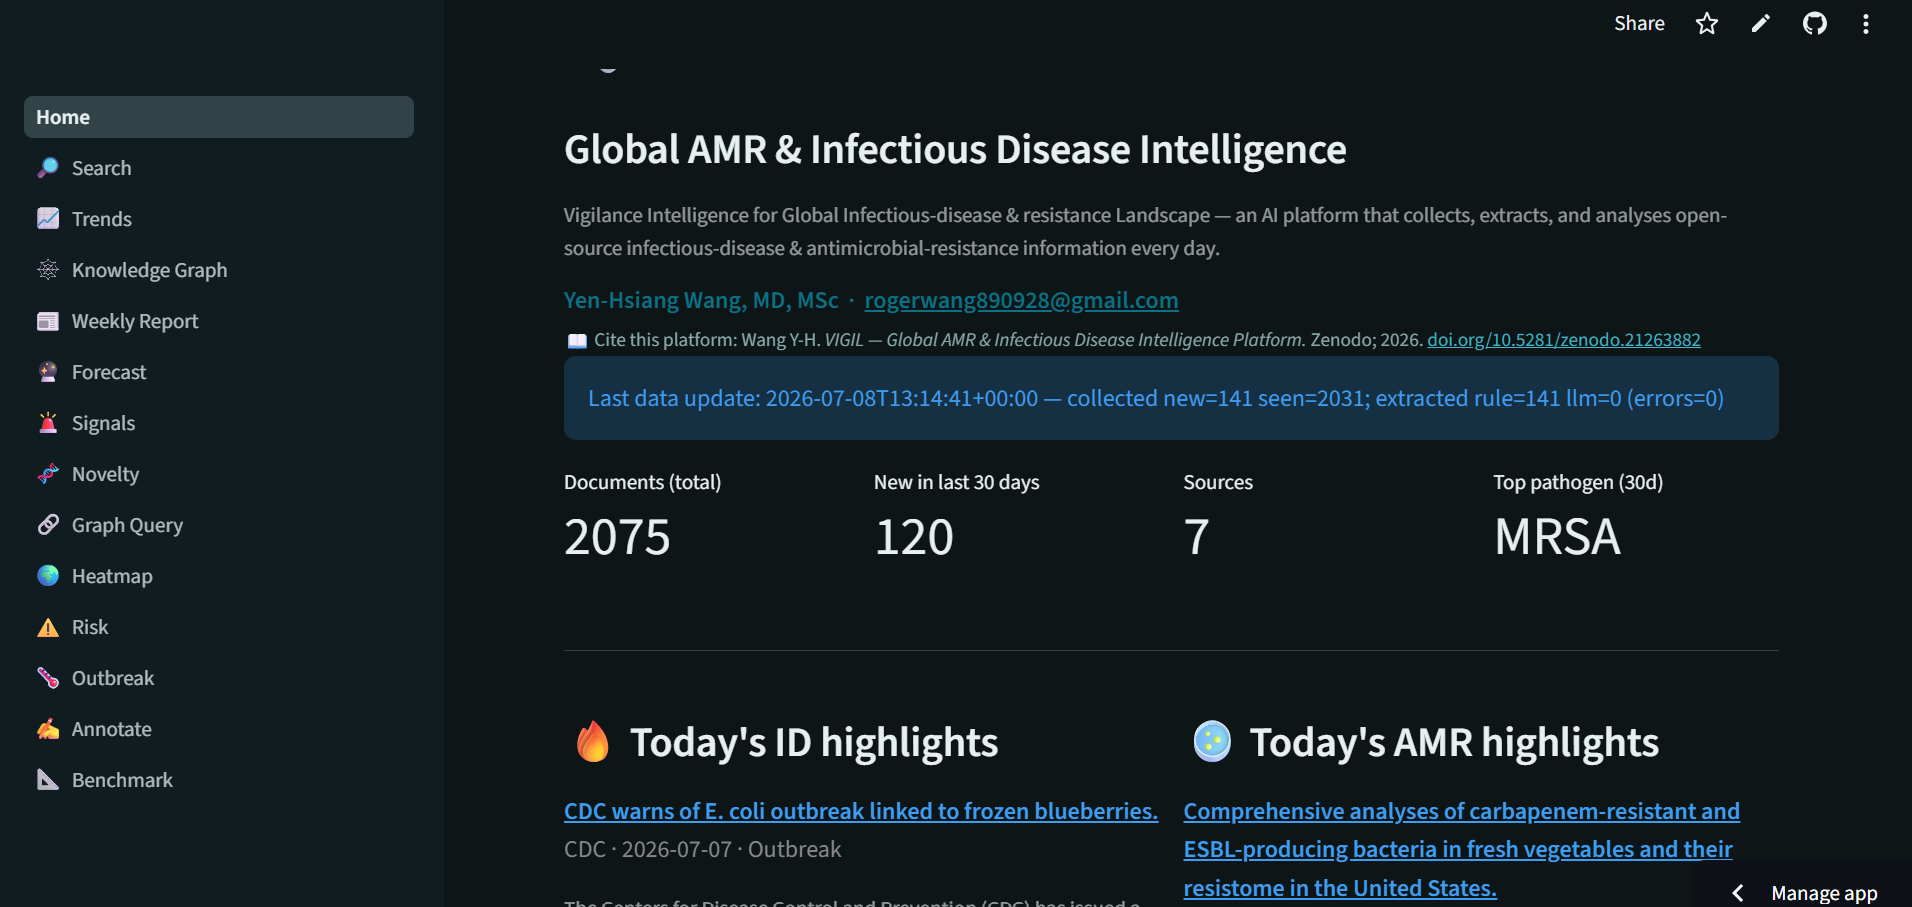
\includegraphics[width=0.78\linewidth]{figure4_dashboard.png}
  \caption{The VIGIL public live instance. Shown for reproducibility and reuse; it is
  the running realisation of the infrastructure in Figure~\ref{fig:arch}, not a
  contribution in itself.}
  \label{fig:dash}
\end{figure}

\end{document}
